As mentioned in \autoref{chapter:fundamentals-of-optics-and-light-microscopy}, the bright-field microscopy images are formed by either transmitted or reflected light that passes through the sample and reach the objective lens. There difference between transmitted light and reflected light microscopes is the illumination system; there is no difference in how both direct light rays after those leave the specimen \cite{leng2009materials}.

According to \citeonline{davidson2002optical}, the light which reaches the specimen is either undeviated, i.e. does not suffer any disturbances in its direction, or diffracted; the diffracted rays leave the sample with a phase difference of 180 degrees in comparison to the undeviated light and cause destructive interference in the eyepiece, which projects a magnified version of this pattern onto a sensor and consequently produces the image.

Furthermore, the diffraction patterns that are captured by objectives have a particular shape. Still as stated by \citeonline{davidson2002optical}, the \emph{Airy disks}(also called \emph{Airy patterns}), named after Sir George Biddell Airy (1801 - 1892), are small circular diffraction disks projected by the objectives onto the image plane of the eyepiece diaphragm, which describe the focus profile the resulting image. The Airy disks as described by \citeonline{fowles1989introduction} follow the Fraunhoffer diffraction pattern, and may be mathematically modelled as an angular distribution of intensity of light diffracted by a circular aperture, given by

\begin{align}
\label{eqn:airy_function}
I(\theta) = I_{0} 
            \left[ 
            \frac{2 J_{1} (\rho)}{\rho}
            \right]^{2}
&&
\rho = \left( 
        \frac{2 \pi \sin{\theta}}{\lambda}
        \right) \frac{a}{2},
\end{align}

\noindent where $I_{0} = (C \pi R^{2})^{2}$ is the intensity for $\theta = 0$, $C$ is a constant, $R$ is the radius of the aperture, $\lambda$ is the wavelength of the light, $a$ is the diameter of the aperture and $J_{1}$ is the Bessel function of the first kind and first order \cite{mathews1970mathematical}, where the general case for the $rth$ order is given by

\begin{align}
\label{eqn:1st_bessel}
J_{r}(x) = \sum_{n = 0}^{\infty}
            \frac{(-1)^{r}}
                 {r! \Gamma(m + r + 1)}
            \left(
                \frac{x}{2}
            \right)^{m + 2r}
&&
\Gamma(z) = \int_{0}^{\infty} e^{-u} u^{z-1}du.
\end{align}

The Airy disks are intrinsically related to the numerical aperture and the definition of \emph{resolution}. The resolution is the minimum distance between two points at which they can be visibly distinguished as two points; optically, it is defined as the minimum distance between two Airy disks that can be distinguished, which is limited by diffraction \cite{leng2009materials}. The resolution of an optical microscope, given by the Rayleigh equation, is described by

\begin{equation}
\label{eqn:resolution}
d = 1.22 \frac{\lambda}{2 NA},
\end{equation}

\noindent where $d$ is the space between two adjacent particles that may be distinguished from each other, $\lambda$ is the wavelength of the illumination and $NA$ is the numerical aperture of the objective \cite{davidson2002optical}. It is evident that objectives with higher numerical apertures and shorter wavelengths of visible light will yield better resolution. \autoref{fig:airy_disks} shows arbitrary examples of Airy patterns, as well as their possible configurations and their consequences to the image. In \autoref{fig:airy_disks}.(a), the usual shape of Airy patterns is shown, together with its two-dimensional representation as a function of the intensity by an interval. Next, \autoref{fig:airy_disks}.(b) depicts an occurrence of Airy disk overlapping where both points would be properly resolved, i.e. below the Rayleigh limit, and \autoref{fig:airy_disks}.(c) represents the minimum distance in which both points would be distinguished. Finally, \autoref{fig:airy_disks}.(d) represents an unresolved pair of points.

\begin{figure}[htb]
	\centering
	\caption{\label{fig:airy_disks} Arbitrary example of an Airy disk (a), resolved Airy disks (b), Rayleigh limit of resolution (c) and unresolved Airy disks (d).} 
	\begin{center}
	    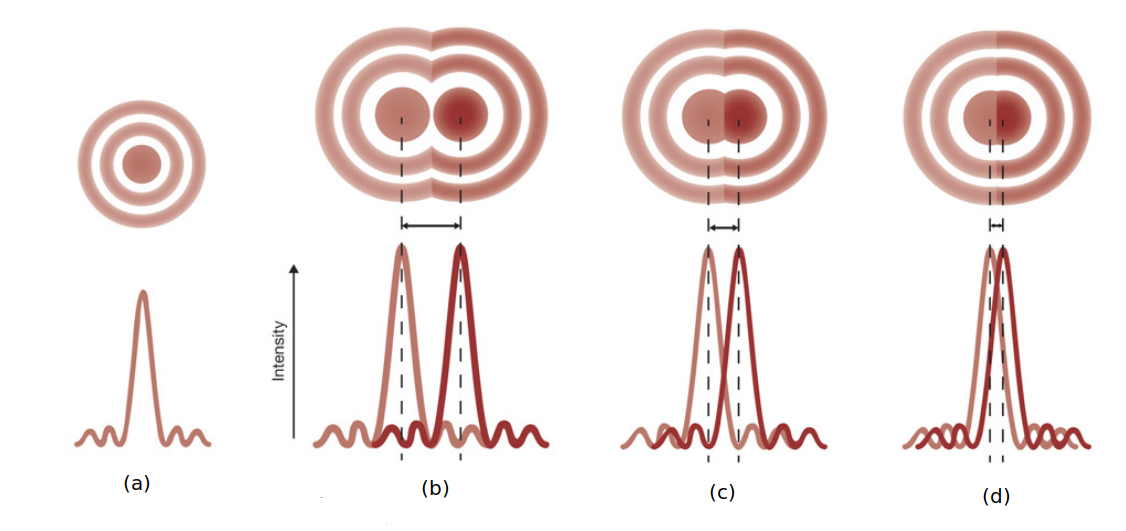
\includegraphics[scale=0.4]{images/airy_disks.png}
	\end{center}
	\centering
    \fadaptada{dunst2019imaging}
\end{figure}

As explained by \citeonline{goodman1996introduction}, an imaging system, particularly a set of microscope lenses, is said to be \emph{diffraction-limited} if the incident spherical light wave generated from a point-source object is transformed into another spherical wave which converges to an ideal image point, described by the original object point and affected by some sort of isotropic effect, such as magnification in a microscope.

The depth of field was described in \autoref{chapter:fundamentals-of-optics-and-light-microscopy} in terms of focal plane distances, but it may also be taken as the \emph{axial resolving power}, a measurement of resolution along the $z$ axis, determined by the numerical aperture and described by the Airy disk profile \cite{davidson2002optical}. Similarly to the Rayleigh's equation, the depth of field increases
with higher numerical apertures for the objective and shorter wavelengths of the incident light, and it represents a key property concerning the amount of blur in the resulting image.


\subsection{Point Spread Function and Image Formation Model}

\label{sec:point_spread_function_and_image_formation_model}

When light waves from a point source reach lenses, they suffer diffraction and refraction, which construct a new propagating set of rays that converge to a point in the center of the image plane in the shape of Airy disks; such shape is called the \sigla{PSF}{Point Spread Function}
of the imaging system (also called \emph{impulse response}), and it is intrinsically related to the imaging process \cite{wu2008microscope}. Particularly, the bright-field microscopy employs polychromatic nonpolarized incoherent light. From this concept, it is possible to relate the Airy disks to the PSF, since those are intensity distributions for each point source of light emanating from the specimen. \autoref{fig:point_spread_function}.(a) presents a theoretical scheme of imaging for a point source of light, and \autoref{fig:point_spread_function}.(b) depicts the shape of a incoherent PSF:

\begin{figure}[htb]
	\centering
	\caption{\label{fig:point_spread_function} Point Spread Function generated by a focused diffraction-limited system with incoherent light.} 
	\begin{center}
	    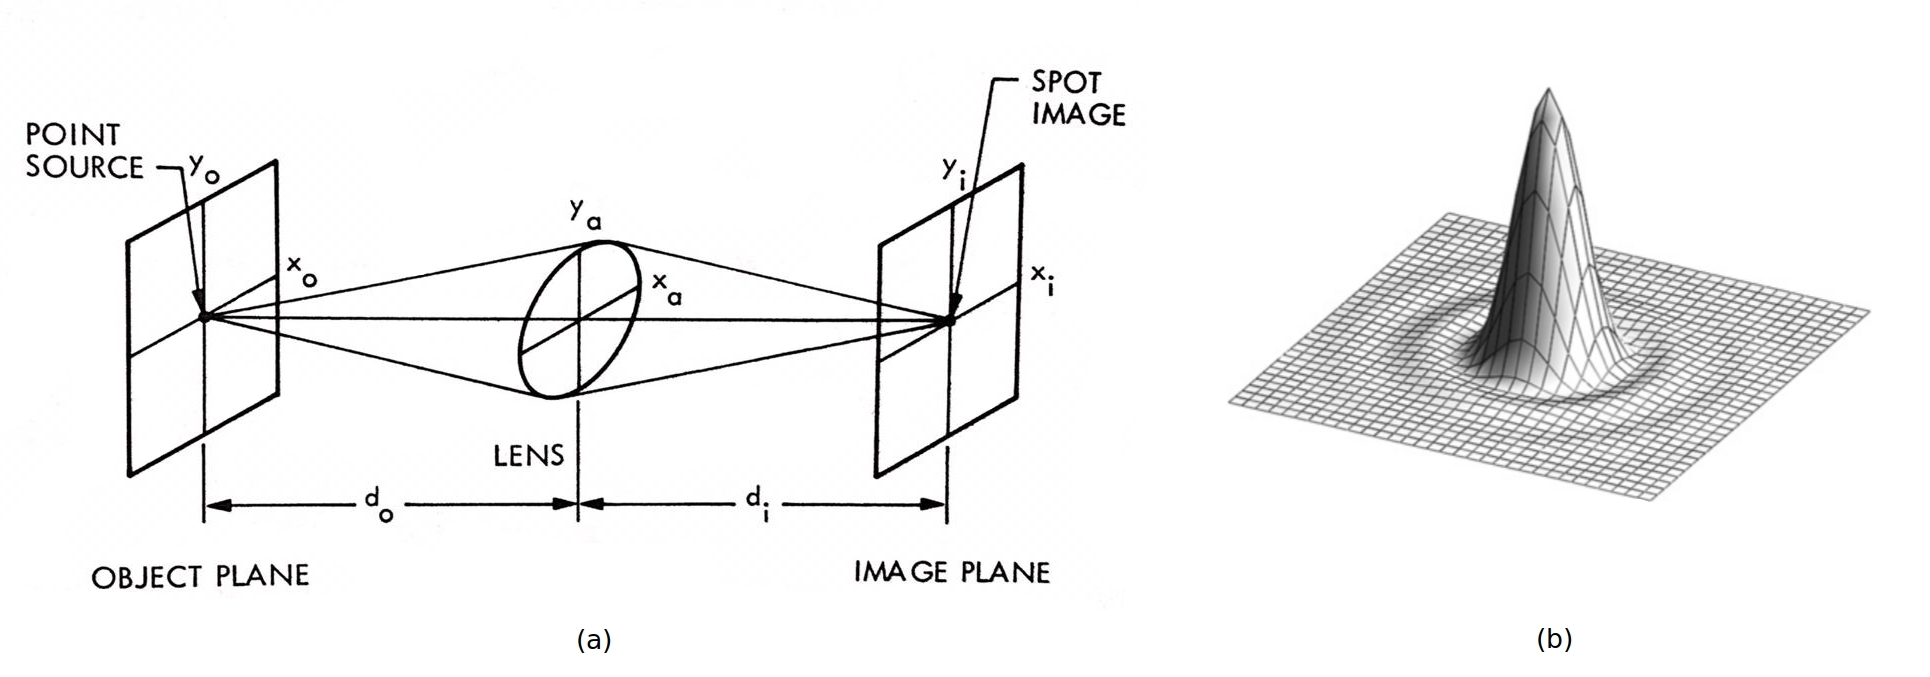
\includegraphics[scale=0.235]{images/point_spread_function.jpeg}
	\end{center}
	\centering
    \fadaptada{castleman1996digital,wu2008microscope}
\end{figure}

In \autoref{fig:point_spread_function}.(a), the imaging system in in focus, which is given by

\begin{equation}
\label{eqn:lens_focus}
\frac{1}{d_{o}} + \frac{1}{d_{i}} = \frac{1}{f},
\end{equation}

\noindent where $f$ is the focal length of the lens, $d_{o}$ and $d_{i}$ are respectively the distances from the point source plane to the lens and the distance from the image plane to the lens; the intensity of light in the point source is directly proportional to the intensity in the image, what characterizes a \emph{two-dimensional linear system} \cite{castleman1996digital}. Still according to \citeonline{castleman1996digital}, any motion of the point source on its plane moves the image is dictated by the law

\begin{align}
\label{eqn:isoplanatic_motion}
x_{i} = -\frac{d_{i}}{d_{o}}x_{o}
&&
y_{i} = -\frac{d_{i}}{d_{o}}y_{o},
\end{align}

\noindent where $(x_{o},y_{o})$ are the coordinates for the object location on its plane and $(x_{i},y_{i})$ are coordinates that locate the image on its plane. This implies that the shape of the image will not change according to the object's location, and this property yield \emph{shift invariance} to the system, which may be called \emph{isoplanatic}. These properties are observed in an ideal imaging system - simple lenses are not isoplanatic and linear, and  consequently simple microscopes also. However, there are approximations and mathematical tools that allow advanced microscopes to be assumed isoplanatic and linear.

The PSF as related to the intensity distributions described by the Airy disks are limited to the area of the aperture. This means that the amount of light that reaches the image plane is truncated by the circular aperture, what is also true for the PSF. The truncation is mathematically represented by the \emph{pupil function}, which is zero outside the boundaries of the aperture and unity otherwise, and might include also information about wave aberrations of the lens \cite{goodman1996introduction}. As denoted by \citeonline{wu2008microscope} with some notation adjustments, the PSF of an incoherent illuminated circular aperture imaging system is the Fourier Transform (explained further in \autoref{chapter:theoretical-background}) of the generalized pupil function, given by

\begin{equation}
\label{eqn:incoherent_psf}
h_{\lambda}(x,y,z) = \int_{-\infty}^{\infty}
                     \int_{-\infty}^{\infty}
         P(u,v)
         e^{j 2 \pi z
            \left(
                \frac{u^{2} + v^{2}}{2 \lambda L^{2}}        
            \right)
        }
        e^{j 2 \pi
            \left(
                \frac{xu + yv}{\lambda L}        
            \right)
        }
        du dv,
\end{equation}

\noindent where $h_{\lambda}(x,y,z)$ is point spread function for a light with wavelength $\lambda$, $P(x,y)$ is the pupil function, $z$ is the axial location the focal plane and $L = r / NA$ is the focal length, i.e. ratio between the radius of the circular aperture of the objective and the numerical aperture. The normalized Fourier Transform of the PSF is called \sigla{OTF}{Optical Transfer Function} \cite{castleman1996digital}.

From this framework, the image is formed as a set of impulse responses from each point in the object plane that where magnified by the imaging system. Linear systems possess a general expression, a convolution (which will be explained in \autoref{chapter:theoretical-background}) of the input with the system's impulse response, that describes the output \cite{brigham1988fast}. In this sense, the resulting image is a convolution of the PSF with the original image, defined as

\begin{equation}
\label{eqn:image_formation_convolution}
g(x,y) = \int_{-\infty}^{\infty}
         \int_{-\infty}^{\infty}
         h(x-u, y-v)f(x,y)du dv,
\end{equation}

\noindent where $f(x,y)$ is the original image, $g(x,y)$ is the observed image, $h(x,y)$ is the PSF of the imaging system and $u,v$ are shift parameters.

\subsection{Discrete Image Formation Model}

Digital images follow a discrete model for image formation due to the acquisition process: the spherical waves that leave the objectives reach the surface of \sigla{CCD}{Charge-coupled Devices}, sensors which proportionally converts light intensities to electrical signals that digitized as pixels \cite{gonzalez2018digital}. The digital images are matrices of pixels that represent light intensities with different channel configurations, where the most common one is the \sigla{RGB}{Red, Green and Blue} image. Therefore, similarly to the image formation model shown in \autoref{sec:point_spread_function_and_image_formation_model}, the two-dimensional digital image formation is described with a discrete process, arbitrarily as

\begin{equation}
\label{eqn:discrete_image_formation}
g[x,y] = h[x,y] \ast f[x,y],
\end{equation}

\noindent where $\ast$ denotes the discrete convolution, $g$, $h$ and $f$ are respectively the observed image, the discrete PSF of the imaging system and the original image, and $x,y \in \mathbb{Z}$. The discrete PSF of an imaging system with incoherent illumination and a circular aperture is given by

\begin{align}
\label{eqn:discrete_psf}
h(r) = \left[
        2
        \frac{J_{1}[\pi (r / r_{0})]}{\pi (r / r_{0})}
       \right]^{2},
&&
r = \sqrt{x^{2} + y^{2}},
&&
r_{0} = \frac{\lambda d_{i}}{a},
\end{align}

\noindent where $h(r)$ is the radially symmetrical PSF, $r$ is the radial distance, $r_{0}$ is a scaling factor, $J_{1}$ is the Bessel function of first order and first kind, $\lambda$ is the wavelength of the illumination, $a$ is the diameter of the aperture and $d_{i}$ is the distance from the lens plane to the image plane. A scheme of the geometric setup of discrete image formation through the PSF is shown in \autoref{eqn:discrete_image_formation}: 

\begin{figure}[htb]
	\centering
	\caption{\label{fig:discrete_psf_scheme} Geometric scheme of a lens' circular aperture and arbitrary point spread function profile.} 
	\begin{center}
	    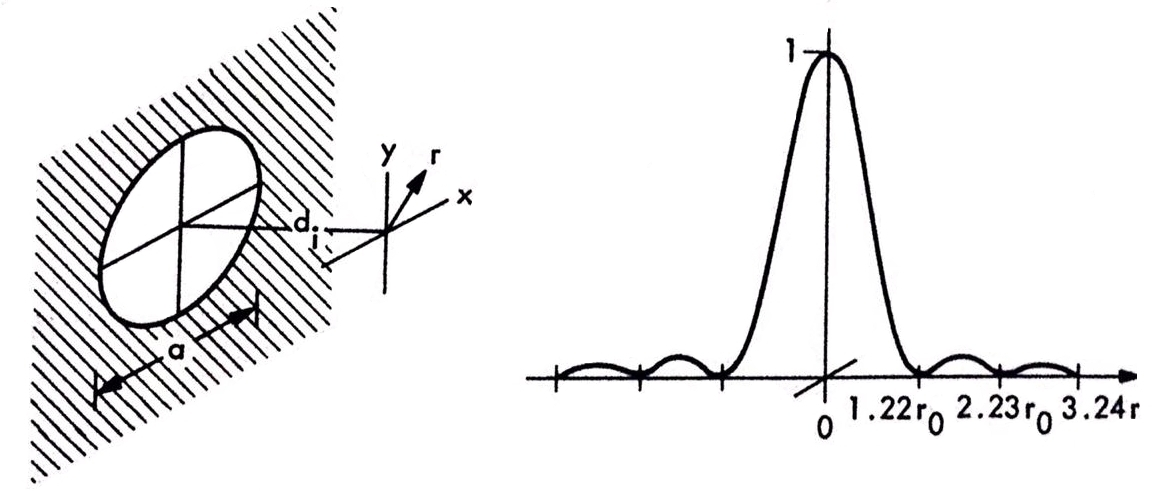
\includegraphics[scale=0.35]{images/discrete_psf_scheme.jpeg}
	\end{center}
	\centering
    \fadaptada{castleman1996digital}
\end{figure}

The discrete OTF is then the \sigla{DFT}{Discrete Fourier Transform} (explained in \autoref{chapter:theoretical-background}) of the PSF in \autoref{eqn:discrete_psf}. The OTF characterizes the intensities of light that emanate from the specimen in terms of frequencies. 

There is another property of image formation and acquisition that influences the image quality: the noise. Pursuant to \citeonline{wu2008microscope}, imaging is corrupted by intrinsic or extrinsic noise; the former is modelled by a Poisson distribution that influences each photon that reaches the sensor, and the latter is modelled by a Gaussian distribution that sums to the matrix of pixels. Details about noise are out of the scope of this work, since the degradation to be deeply explored is the defocus blur.